\documentclass[12pt]{article}
\usepackage[margin=1in]{geometry}
\usepackage{setspace}
\usepackage{amsmath,textcomp,amssymb,geometry,graphicx,enumerate}
\usepackage{mathtools, dsfont}
\usepackage{fancyvrb, color}
\usepackage{grffile}
\DeclarePairedDelimiter\ceil{\lceil}{\rceil}
\DeclarePairedDelimiter\floor{\lfloor}{\rfloor}

\textheight=9in
\textwidth=6.5in
\topmargin=-.75in

\begin{document}
\setcounter{MaxMatrixCols}{20}
\setlength\parindent{0pt}

\textbf{\underline{Panhandler's Bus Fee}}\\

You want to go home but the 8 dollars you have in your pocket are not enough to cover the 12 dollar bus fare. Because you happen to be near Las Vegas, you decide to fix your problem by gambling.\\

The game you play is structured as follows: in each turn, you bet some amount of money and a wheel is spun. If the wheel lands on a good sector, you gain the amount of money you bet. If not, you lose the amount of money you bet. On this wheel, you have probability $\frac{9}{19}$ of winning a turn.\\

You decide to play The Best Strategy with a goal of 10 dollars in mind. That is, at each turn, you bet as much money as you can to reach 10 dollars in one turn. For example, if you have 6 dollars, you would bet 4 dollars so that you would either win the game or you would have to take another turn with 2 dollars leftover.\\

Collecting 10 total dollars means that you "win a game", whereas losing all the money you start out with means you "lose a game". If you win a game, you replay the game with the same strategy starting with 8 dollars, saving the rest of whatever amount you currently have. Losing a game here means that you lose the 8 dollars you start out with; you stop playing when this happens.\\

{\color{blue} What is the probability of amassing 12 dollars before losing a game?}\\

\textbf{Solution:} Recall the following graph. The green arrows signify that you would restart the game with 8 dollars out of your current sum of money if you hit the 10 dollar goal in your current game.
\begin{center}
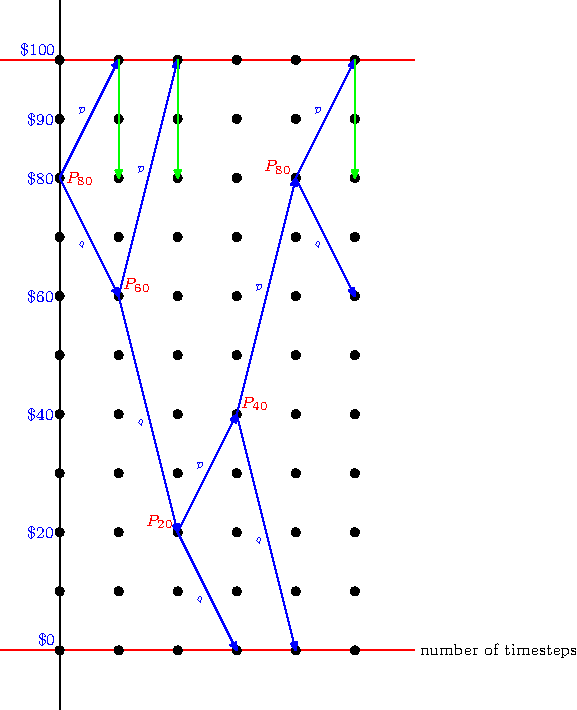
\includegraphics[scale=0.9]{126figs-9.pdf}
\end{center}

Collecting 12 total dollars would occur only if you win two consecutive games, because each game gives you a gain of 2 dollars.\\

Denote $p_{i,j}$ to be the probability of collecting 12 dollars when you have $i$ dollars of betting money in your current game and you have $j$ saved dollars in your pocket. The value we desire is $p_{8,0}$. Assume for simplicity that $p_{0, j} = 0$ for all $j$, i.e, if you lose the game, you stop playing no matter how much money you have saved. We will get rid of this assumption later on. {\color{red} reflecting boundary} \\

First, we must consider all possible sample paths in order to determine what numbers $i$ and $j$ will take. Let $W$ denote the event that you win a turn and $L$ denote the event of a loss. Let $\Omega_{i, j}$ denote the set of all possible sample paths starting from $i$ dollars betting and $j$ dollars saved. We will only use $i = 8$ and enumerate all other cases.\\

Build $\Omega_{8, 2}$. Then the best case scenario is when you win the game first turn: that is, you get from $\{8, 2\}$ to $\{8, 4\}$. And $p_{8, 4} = 1$ because you can get 12 dollars from combining your betting money (8) and your saved money (4). As a sample path, we shall denote this $W$.\\

Suppose you lost the first turn. Then you get from $\{8, 2\}$ to $\{6, 2\}$. From there, multiple sample paths would arise. We list them all as follows:
\begin{align*}
\{6, 2\} \rightarrow \{8, 4\} &\Longrightarrow LW\\
\{6, 2\} \rightarrow \{2, 2\} \rightarrow \{0, 2\} &\Longrightarrow LLL\\
\{6, 2\} \rightarrow \{2, 2\} \rightarrow \{4, 2\} \rightarrow \{0, 2\} &\Longrightarrow LLWL\\
\{6, 2\} \rightarrow \{2, 2\} \rightarrow \{4, 2\} \rightarrow \{8, 2\} &\Longrightarrow LLWW
\end{align*}

Note that in the last case, you end up back at $\{ 8, 2\}$. From there it is just a recursive repeat of sample paths. We will encompass this using the notation $LLWW\Omega_{8, 2}$.

Overall,
\begin{align*}
\Omega_{8, 2} = \left\{ W, LW, LLL, LLWL, LLWW\Omega_{8, 2} \right\}
\end{align*}

Now build $\Omega_{8, 0}$. Best case scenario is that you win the first game in one turn. Then you get from $\{8, 0\}$ to $\{8, 2\}$, from which $\Omega_{8, 2}$ encompasses all the possible sample paths.\\

If you instead lost the first turn ($\{8, 0\} \rightarrow \{6, 0\}$), we similarly list all the sample paths that arise:
\begin{align*}
\{6, 0\} \rightarrow \{8, 2\} &\Longrightarrow LW\Omega_{8, 2}\\
\{6, 0\} \rightarrow \{2, 0\} \rightarrow \{0, 0\} &\Longrightarrow LLL\\
\{6, 0\} \rightarrow \{2, 0\} \rightarrow \{4, 0\} \rightarrow \{0, 0\} &\Longrightarrow LLWL\\
\{6, 0\} \rightarrow \{2, 0\} \rightarrow \{4, 0\} \rightarrow \{8, 0\} &\Longrightarrow LLWW\Omega_{8, 0}
\end{align*}

Overall,
\begin{align*}
\Omega_{8, 0} = \left\{ W\Omega_{8, 2}, LW\Omega_{8, 2}, LLL, LLWL, LLWW\Omega_{8, 0} \right\}
\end{align*}

Now we can set up equations for the probabilities that correspond to these sample paths. We have that $p_{8, 0} = P\left( \Omega_{8, 0}\right)$, $p_{8, 2} = P\left( \Omega_{8, 2}\right)$, and
\begin{align*}
p_{8, 0} &= P\left( W\Omega_{8, 2}\right) + P\left( LW\Omega_{8, 2}\right) + P\left( LLL\right) + P\left( LLWL\right) + P\left(  LLWW\Omega_{8, 0}\right)\\
&= \frac{9}{19}p_{8, 2} + \frac{10}{19}*\frac{9}{19}p_{8, 2} + 0 + 0 + \frac{10}{19}*\frac{10}{19}*\frac{9}{19}*\frac{9}{19}*p_{8, 0}
\end{align*}

Similarly for $\Omega_{8, 2}$:
\begin{align*}
p_{8, 2} &= P\left( W\right) + P\left( LW\right) + P\left( LLL\right) + P\left( LLWL\right) + P\left(  LLWW\Omega_{8, 2}\right)\\
&= \frac{9}{19} + \frac{10}{19}*\frac{9}{19} + 0 + 0 + \frac{10}{19}*\frac{10}{19}*\frac{9}{19}*\frac{9}{19}*p_{8, 2}
\end{align*}

We can solve this system of equations to get the following results:
\begin{align*}
p_{8, 0} &= 0.5943\\
p_{8, 2} &= 0.7709
\end{align*}
and so you have a 59.43$\%$ chance of getting 12 dollars before you lose.\\

% Now we can set up equations for the probabilities that correspond to these sample paths. 

% From 8 dollars, you bet 2 dollars. Either you get 10 dollars with probability $\frac{9}{19}$ (from which you restart the game with $j = 2$) or you have 6 dollars left over with probability $\frac{10}{19}$.
% \begin{align*}
% p_{8, 0} = \frac{9}{19}p_{8, 2} + \frac{10}{19}p_{6, 0}
% \end{align*}

% Similarly for when you already have 2 dollars saved in your pocket:
% \begin{align*}
% p_{8, 2} &= \frac{9}{19}p_{8, 4} + \frac{10}{19}p_{6, 2}\\
% &= \frac{9}{19} + \frac{10}{19}p_{6, 2}
% \end{align*}
% where $p_{8, 4} = 1$ since you can get 12 dollars from combining your betting money and your saved money.\\

% When you have 6 dollars, you bet 4 dollars. Either you get 10 dollars (from which you restart the game with 8 dollars, with 2 dollars saved), or you are left with 2 dollars:
% \begin{align*}
% p_{6, 0} = \frac{9}{19}p_{8, 2} + \frac{10}{19}p_{2, 0}
% \end{align*}

% Similarly for when you are in this situation with 2 dollars saved:
% \begin{align*}
% p_{6, 2} &= \frac{9}{19}p_{8, 4} + \frac{10}{19}p_{2, 2}\\
% &= \frac{9}{19} + \frac{10}{19}p_{2, 2}
% \end{align*} 

% When you have 2 dollars, you bet all you have. Then:
% \begin{align*}
% p_{2, 0} &= \frac{9}{19}p_{4, 0} + \frac{10}{19}p_{0, 0}\\
% &= \frac{9}{19}p_{4, 0}
% \end{align*}
% where $p_{0, 0} = 0$ because you have no more money to bet and you can no longer play the game.\\

% Similarly for when you have 2 and 4 dollars saved:
% \begin{align*}
% p_{2, 2} &= \frac{9}{19}p_{4, 2} + \frac{10}{19}p_{0, 2}\\
% p_{2, 4} &= \frac{9}{19}p_{4, 4} + \frac{10}{19}p_{0, 4}
% \end{align*}

You've successfully amassed 12 dollars, so you walk to the bus station. However, you find that the bus fare has been raised to 14 dollars. You don't want to walk the long distance back to your casino again, so you settle for panhandling on the street. The time is currently 7:30pm. \\

The people who pass by you can be modeled as a Poisson process with rate 3 per minute. Each person will toss you 50 cents with probability $\frac{1}{10}$. The next bus to take you home is scheduled to arrive at 7:35pm.\\

{\color{blue} What is the probability that you will have collected a total of 14 dollars by the time the next bus arrives?}\\

\textbf{Solution:} 

\end{document}